%! TEX root = **/000-main.tex
% vim: spell spelllang=en:

\subsection{Non-Normalized arcsine kernel}

Now, we will introduce the non-normalized arcsine kernel, and compare it with
both the normalized arcsine kernel and the radial basis kernel.

\subsubsection{Regression}



\begin{figure}[H]
    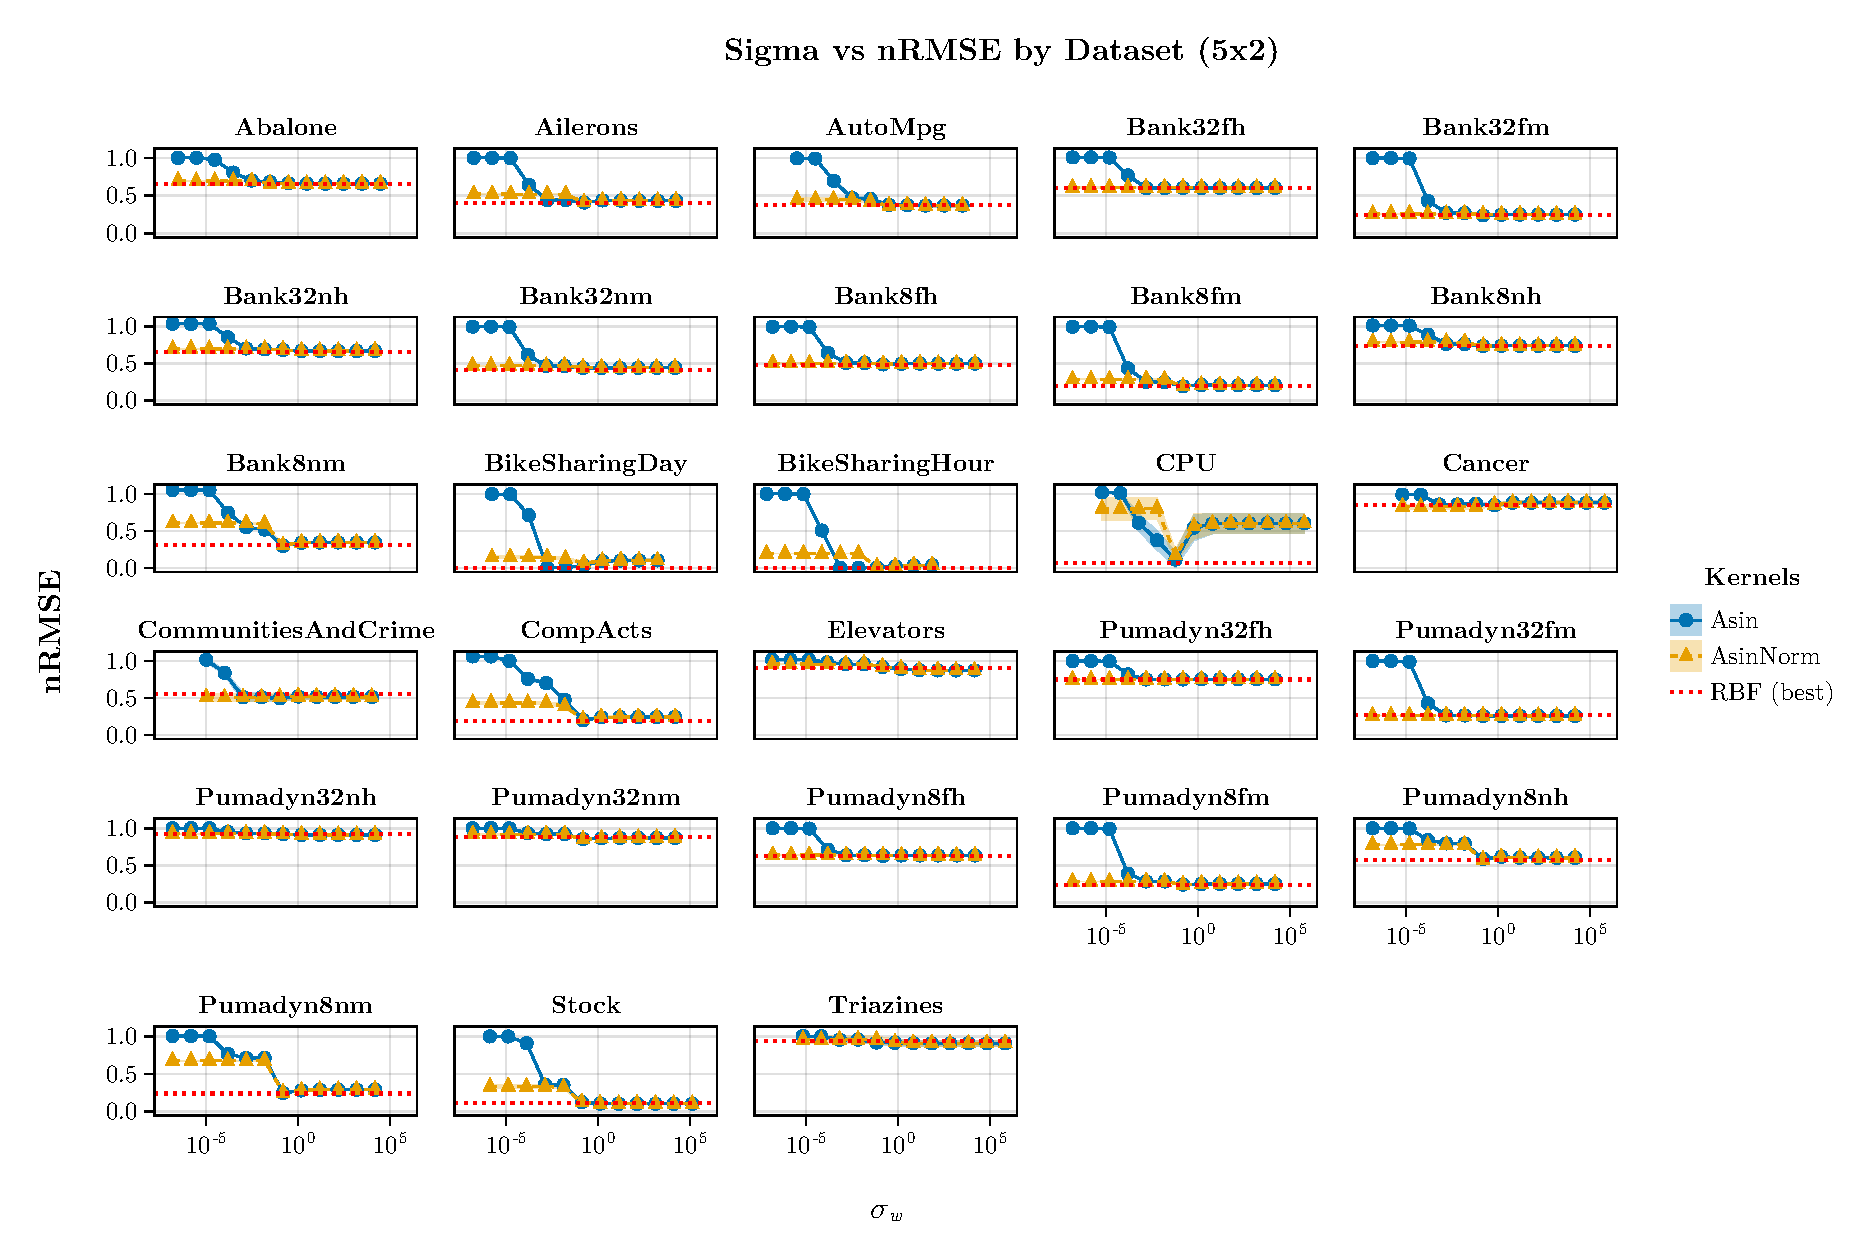
\includegraphics{plots/nRMSE_all_scaled}
    \caption{Sigma vs Normalized Root Mean Squared error by dataset using Normalized arcsine kernel}%
    \label{fig:nrmse-all-scaled}
\end{figure}

\begin{figure}[H]
    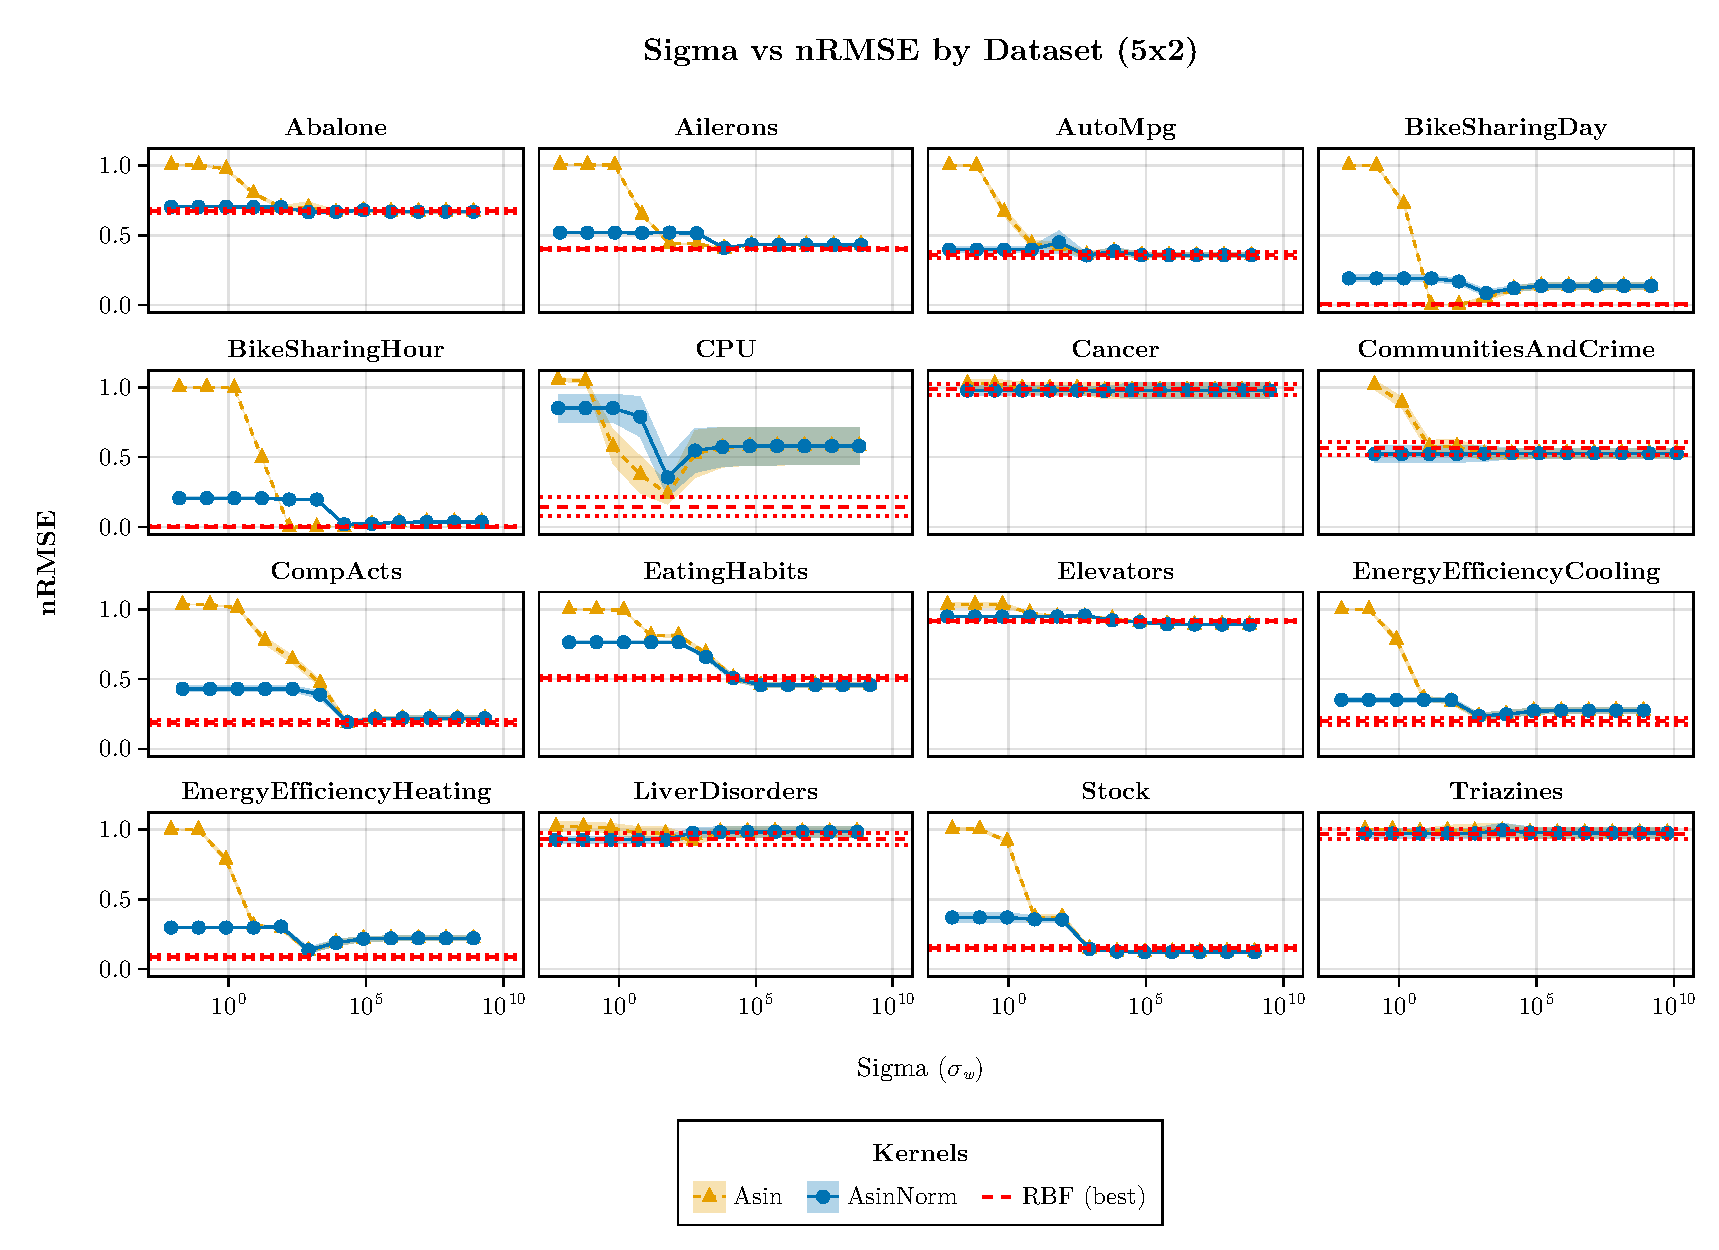
\includegraphics{plots/nRMSE_nodelve_all_scaled}
    \caption{Sigma vs Normalized Root Mean Squared error by dataset using Normalized arcsine kernel}%
    \label{fig:nrmse-all-scaled}
\end{figure}

\paragraph{Bank Delve Dataset}

% TODO: Facet all delve datasets into a single one.

\begin{figure}[H]
    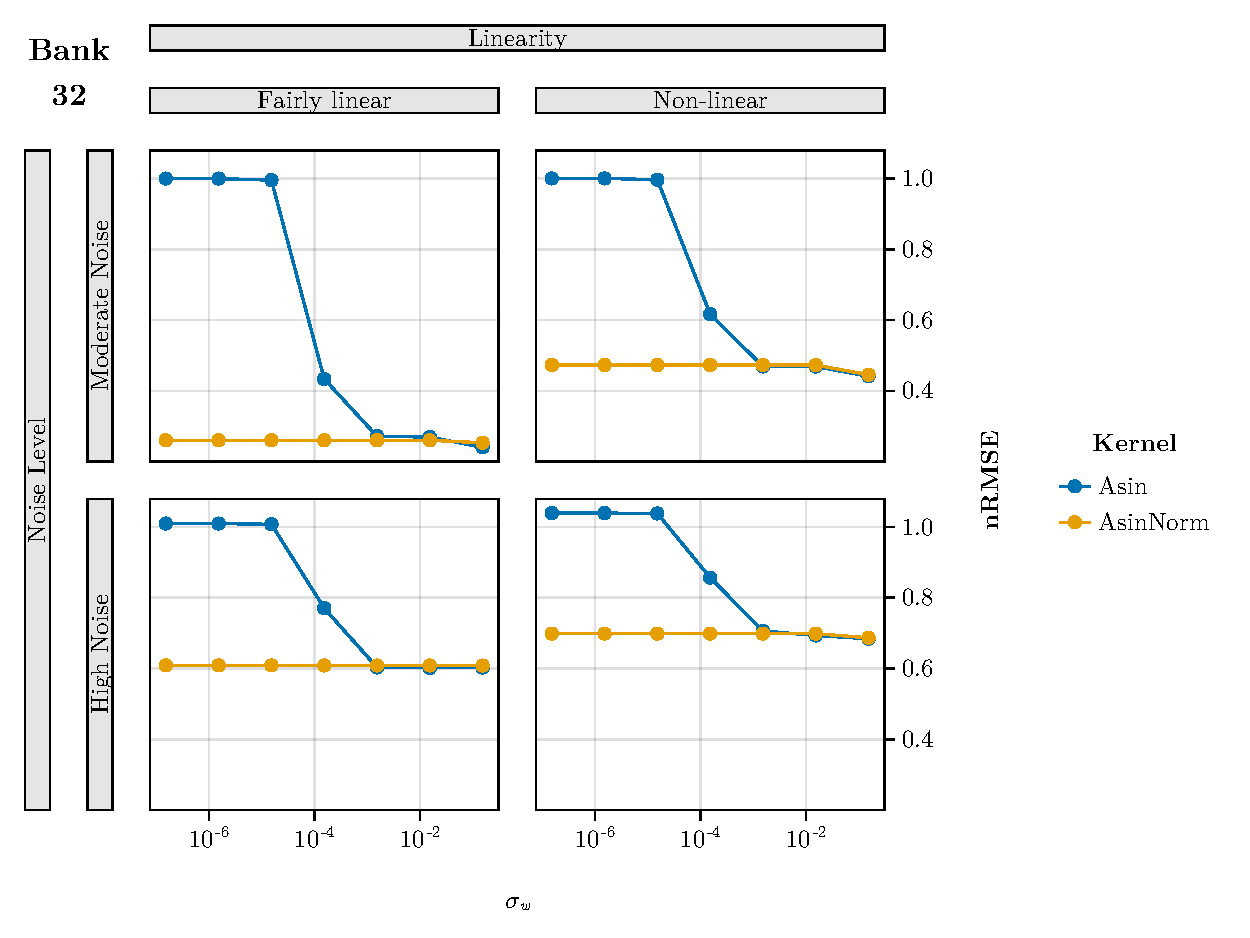
\includegraphics[width=0.7\textwidth]{plots/nRMSE_delve_bank_32_scaled}
    \caption{nRMSE results on Delve Bank32 dataset with $\sigma_w$ scaled}
    \label{fig:nrmse-delve-all-bank-32-scaled}
\end{figure}

\begin{figure}[H]
    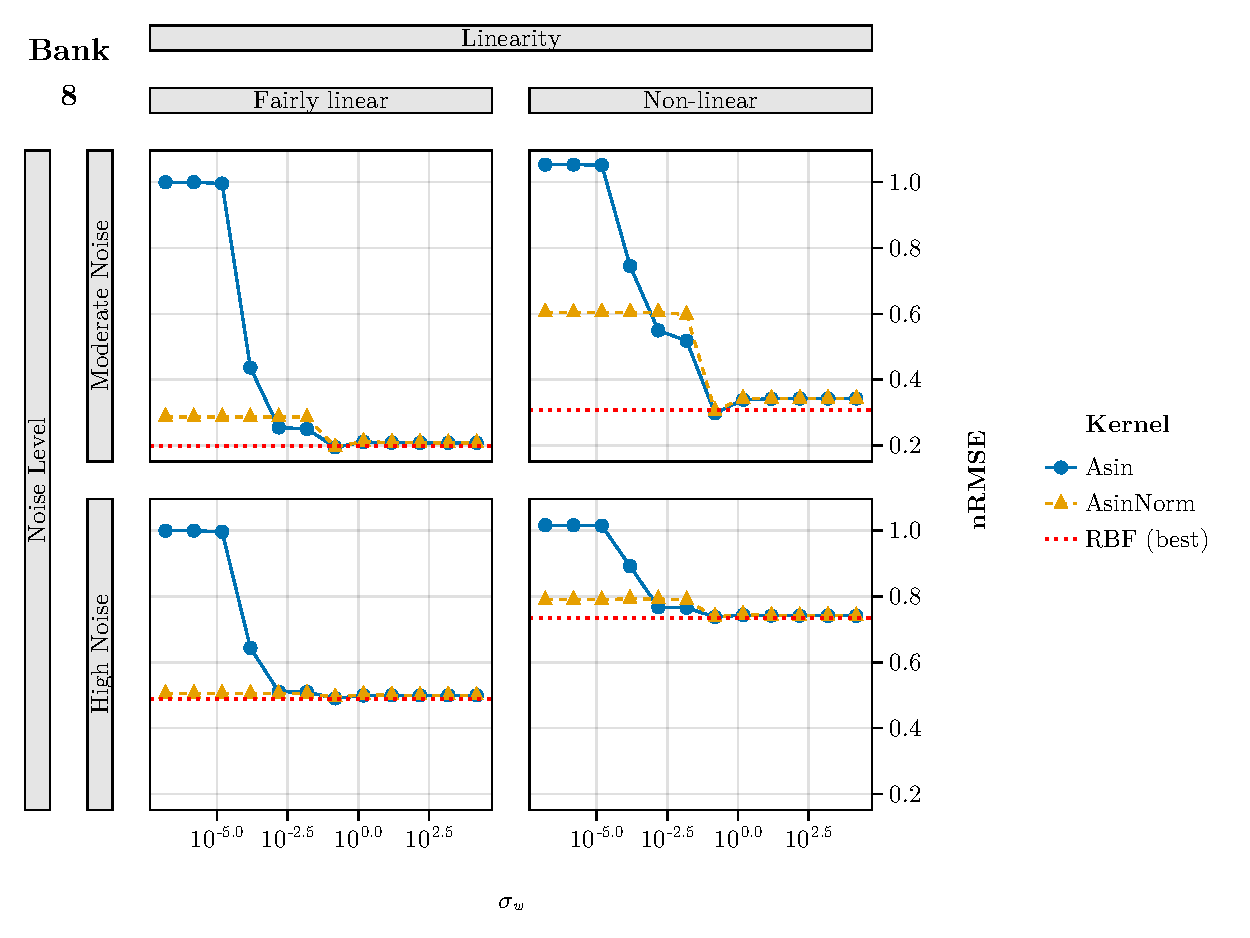
\includegraphics[width=0.7\textwidth]{plots/nRMSE_delve_bank_8_scaled}
    \caption{nRMSE results on Delve Bank8 dataset with $\sigma_w$ scaled}
    \label{fig:nrmse-delve-bank-8-scaled}
\end{figure}


\paragraph{Pumadyn Delve Dataset}

\begin{figure}[H]
    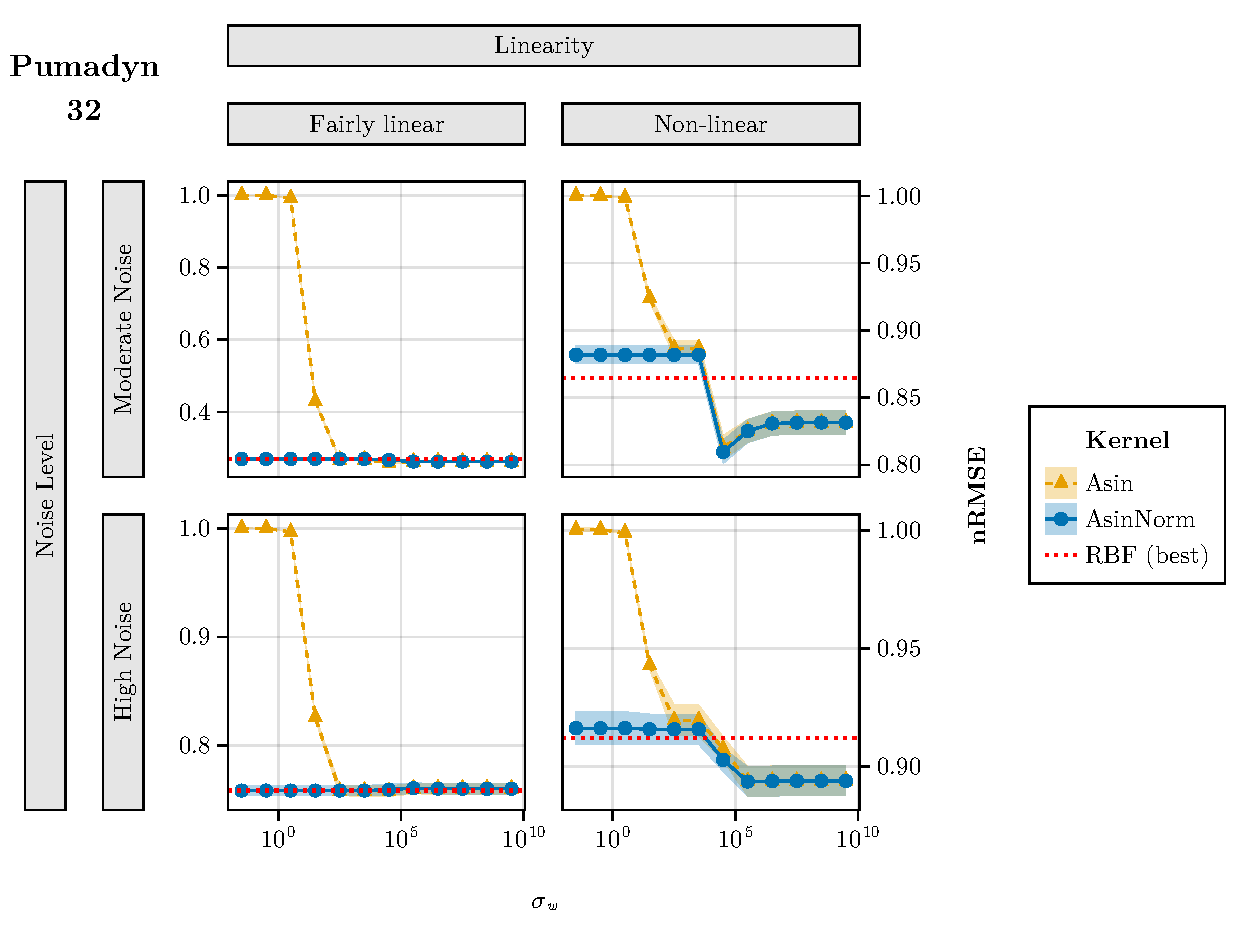
\includegraphics[width=0.7\textwidth]{plots/nRMSE_delve_pumadyn_32_scaled}
    \caption{nRMSE results on Delve PumaDyn32 dataset with $\sigma_w$ scaled}
    \label{fig:nrmse-delve-pumadyn-32-scaled}
\end{figure}

\begin{figure}[H]
    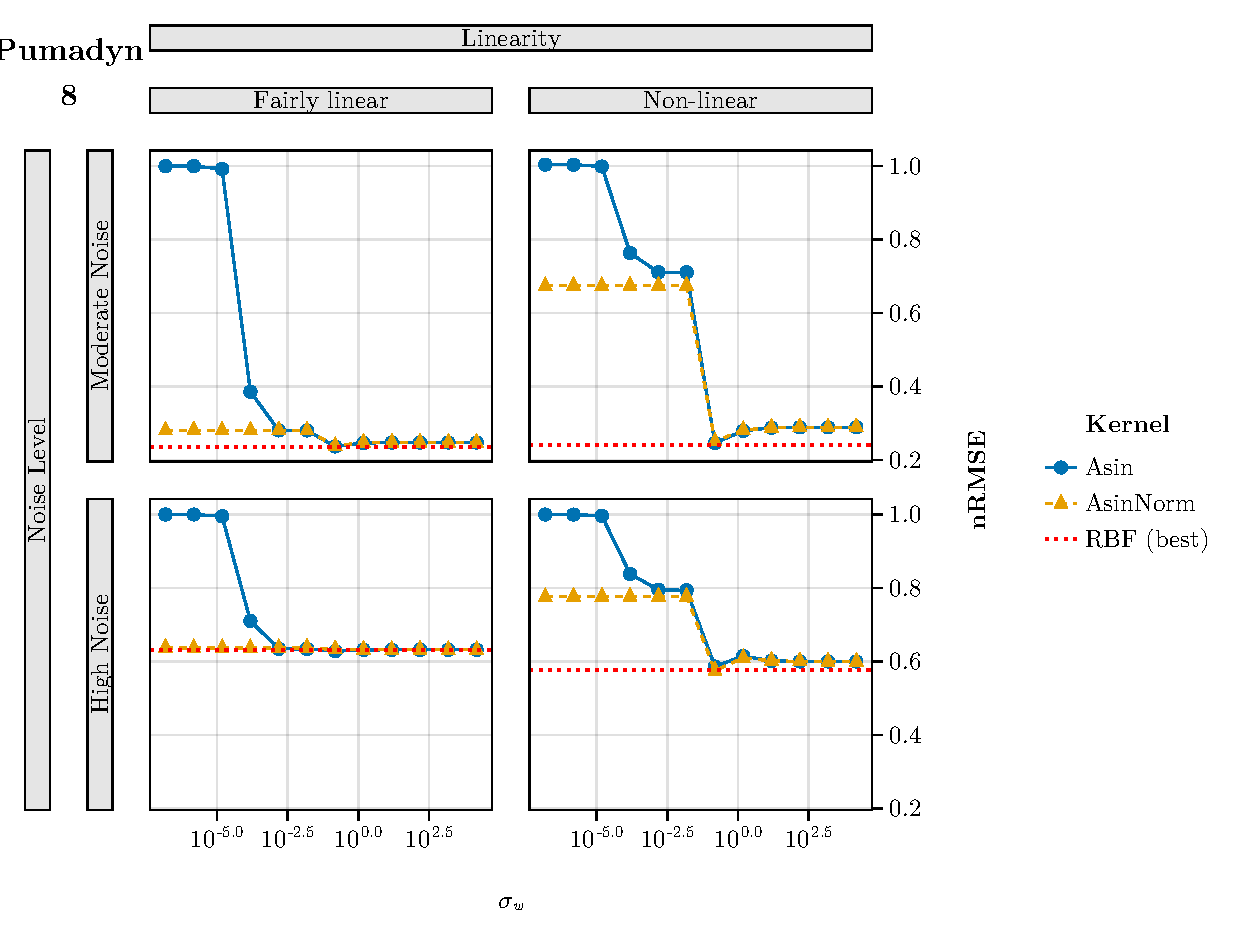
\includegraphics[width=0.7\textwidth]{plots/nRMSE_delve_pumadyn_8_scaled}
    \caption{nRMSE results on Delve PumaDyn8 dataset with $\sigma_w$ scaled}
    \label{fig:nrmse-delve-asinnorm-pumadyn-8-scaled}
\end{figure}

\subsubsection{Classification}

\begin{figure}[H]
    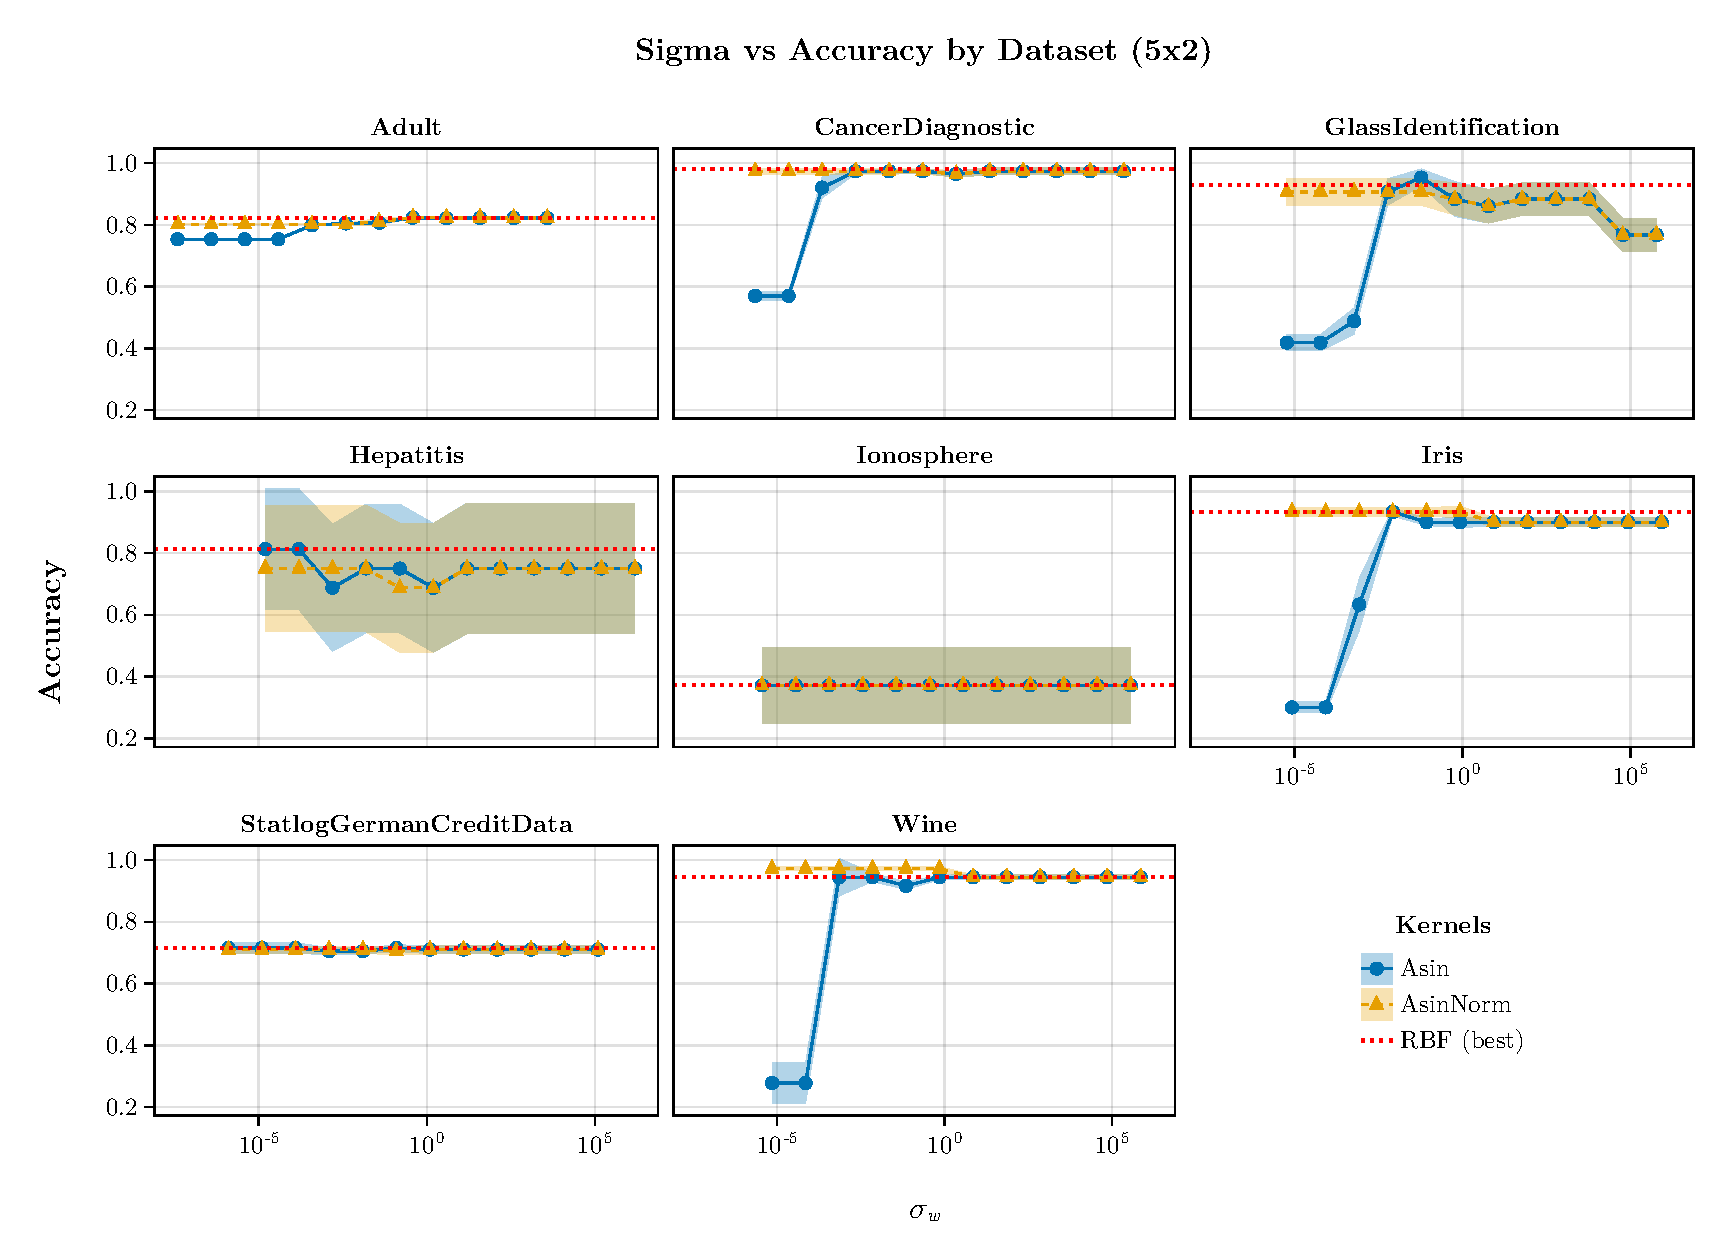
\includegraphics{plots/accuracy_class_all_scaled}
    \caption{Sigma vs Accuracy by dataset using Normalized arcsine kernel}%
    \label{fig:accuracy-asinnorm-scaled}
\end{figure}

\subsubsection{Comparison with radial basis (RBF) kernel}

\begin{figure}[H]
    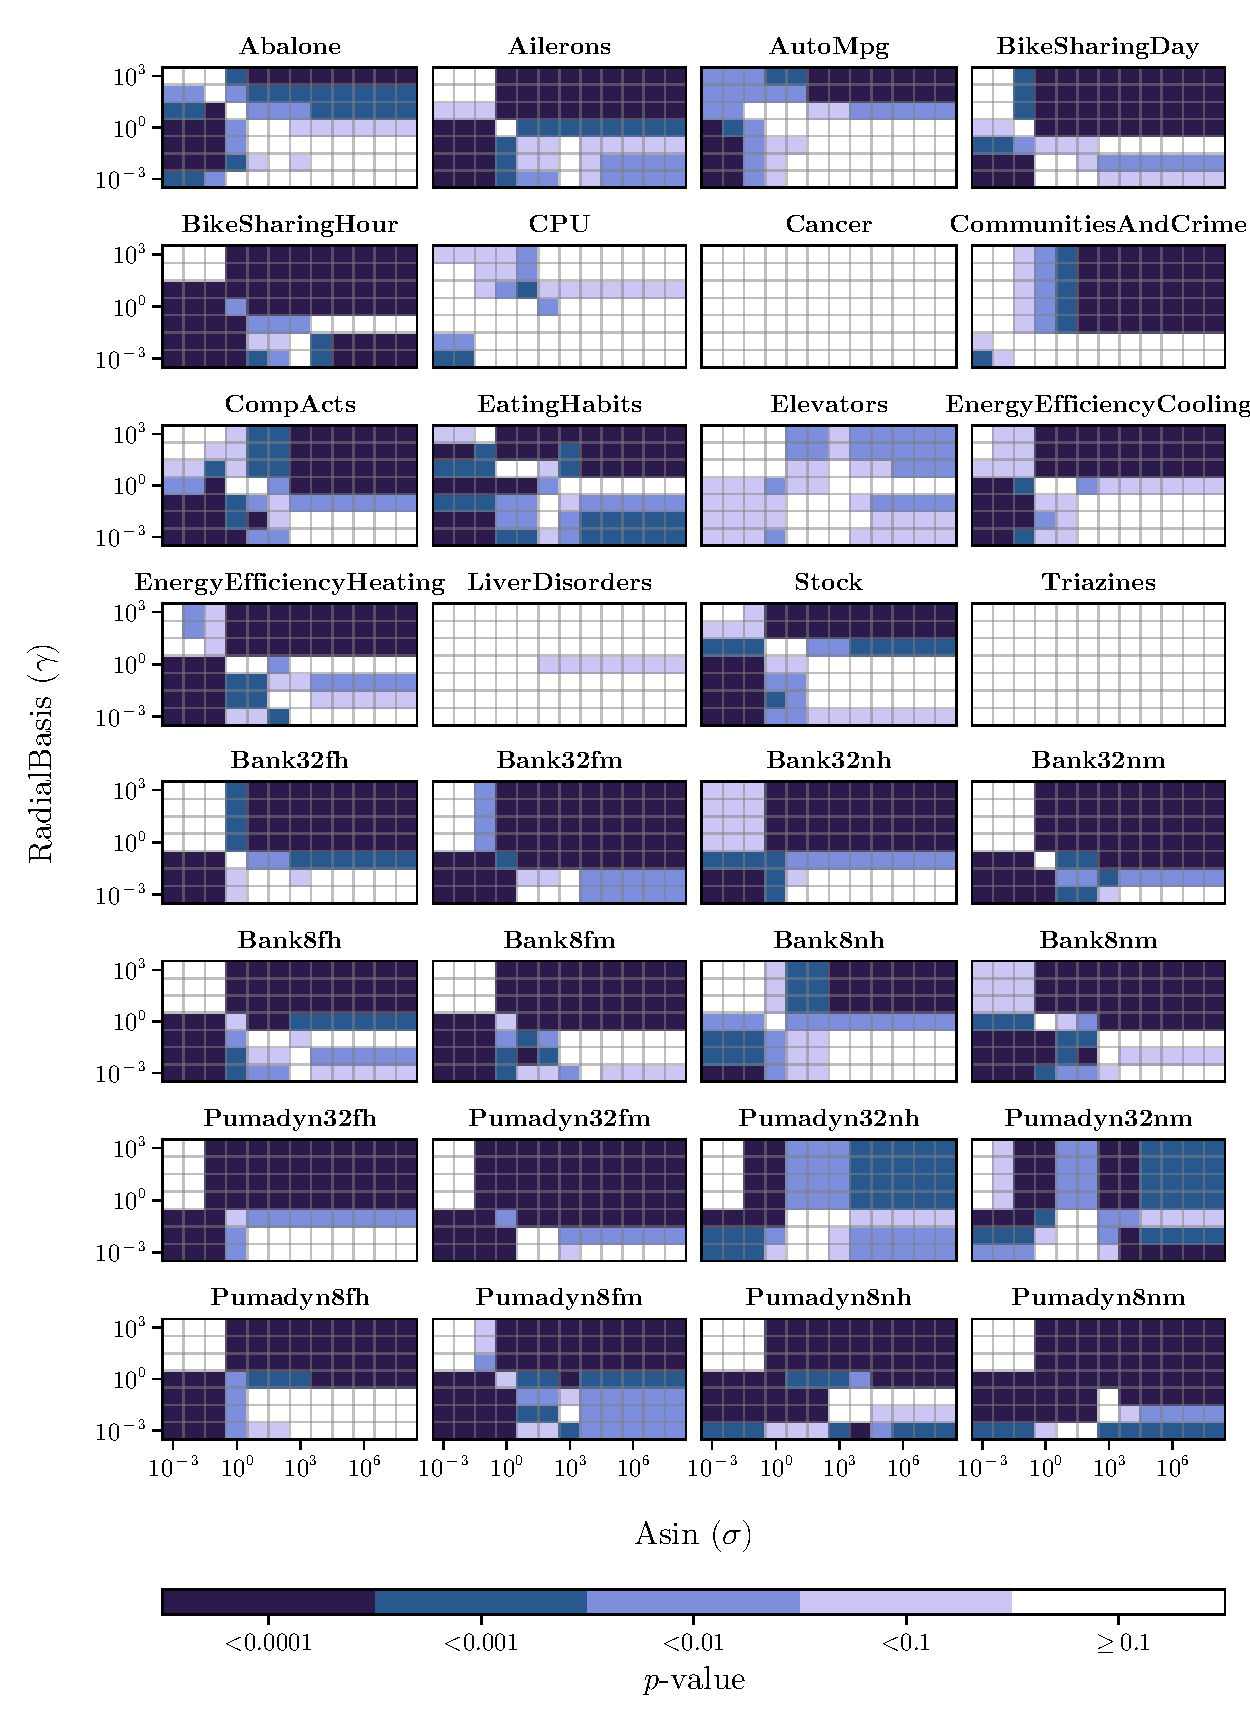
\includegraphics[width=0.9\textwidth]{plots/heatmaps_rbf_asin_pvalues}
    \caption{p values}
    \label{fig:paired-ttest-rbf-asinnorm}
\end{figure}

%  TODO: add pattern or something so the color can be seen in b/w
\begin{figure}[H]
    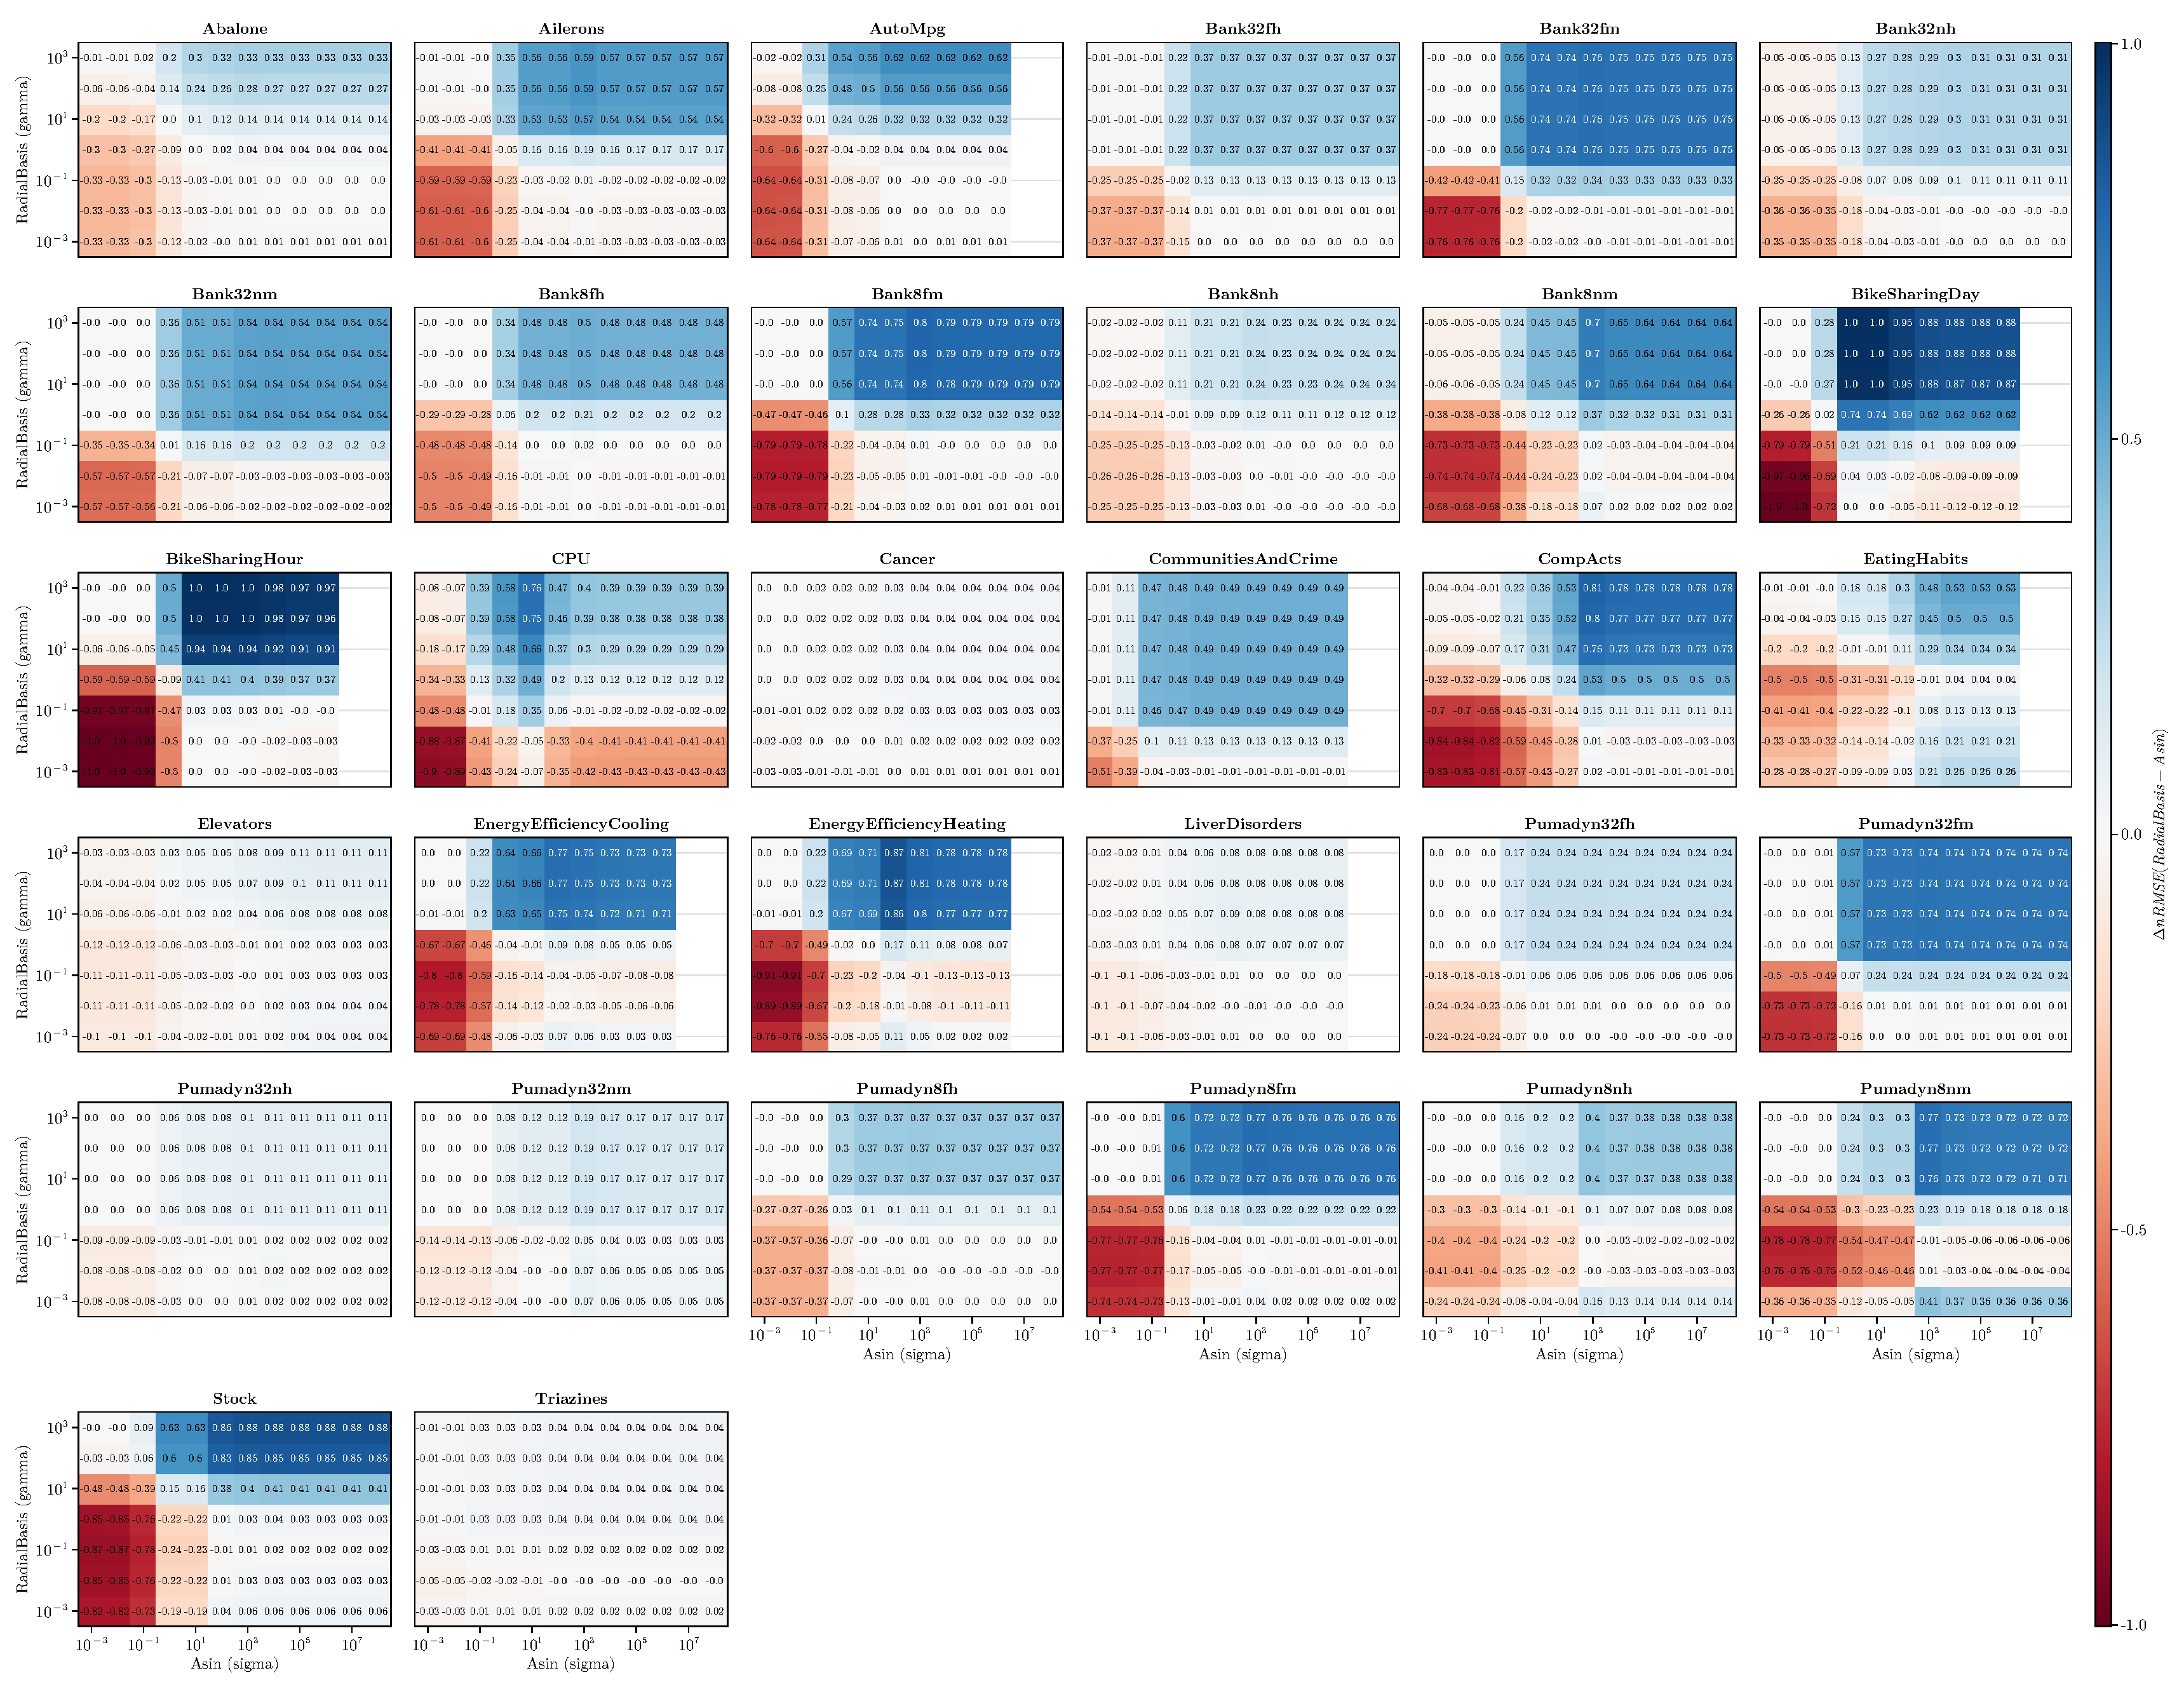
\includegraphics[width=0.9\textwidth]{plots/heatmaps_rbf_asin}
    \caption{Difference between nRMSE of RBF and normalized arc-sine kernels ($\alpha=0.001$)}
    \label{fig:paired-ttest-rbf-asinnorm-diff}
\end{figure}

\subsubsection{Computational Cost}
